
\documentclass[12pt]{article}
\usepackage{amsmath}
\newcommand{\myvec}[1]{\ensuremath{\begin{pmatrix}#1\end{pmatrix}}}
\newcommand{\mydet}[1]{\ensuremath{\begin{vmatrix}#1\end{vmatrix}}}
\newcommand{\solution}{\noindent \textbf{Solution: }}
\providecommand{\brak}[1]{\ensuremath{\left(#1\right)}}
\providecommand{\norm}[1]{\left\lVert#1\right\rVert}
\let\vec\mathbf
\usepackage{graphicx}
\begin{document}

\title{Coordinate-Geomentry}
\author{sai charvi(PATNANASAICHARVI@sriprakashschools.com)}

\begin{document}
\maketitle
\section*{10$^{th}$ Maths - Chapter 7}
This is Problem-1 from Exercise 7.2
\begin{enumerate}
\item Find the coordinates of the point which divides the join of (–1, 7) and (4, –3) in the
ratio 2 : 3\\
\end{enumerate}
\solution \\
Given,\\
$\vec{A}$=\myvec{-1\\7}, $\vec{B}$=\myvec{4\\-3},
$m_1:m_2=2:3$
\begin{align}
\myvec{P}=\frac{m_1\vec{B}+m_2\vec{A}}{m_1+m_2}\\
&=\frac{2\myvec{4\\-3}+4\myvec{-1\\7}}{2+3}\\
&=\frac{\myvec{8-3\\-6+21}}{2+3}\\
&=\myvec{\frac{8-3}{2+3}\\\frac{-6+21}{2+3}}\\
&=\myvec{\frac{5}{5}\\\frac{15}{5}}
\end{align}
\begin{figure}[H]
			\centering
			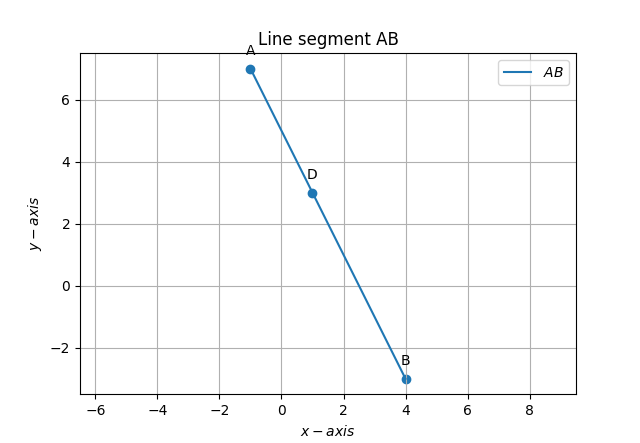
\includegraphics[width=\columnwidth]{figs/Figure_1.png}
			\caption{Line segment AB}
			\label{fig:12}
		\end{figure}

\end{document}
